\section{Identification of the size of the informal sector}

This section uses the model without the earnings observable to show what aggregate data can say about the level of the informal share, and then introduces the observable that identifies it. The evidence is reported for the equal-technology model, where the mechanism is transparent; the labor-only technology does not change the conclusion (Section~\ref{sec:alt-tech}).
\label{sec:identification}

\subsection{Where information about the level can come from}

Section~\ref{sec:model} shows that steady-state ratios are consistent with any value of $\theta$. In the log-linearized equal-technology model, $\theta$ enters the dynamics only through the weights of the two types of work in effective labor,
\begin{equation}
d\ln L_t = (1-\theta)\,d\ln N_{f,t} + \theta\,d\ln N_{i,t},
\label{eq:effective}
\end{equation}
so the only source of information is the co-movement of output with the composition of employment. When the wedge moves workers between sectors, output changes more if informal work is much less productive than formal work (small $\theta$) and less if the two are similar (large $\theta$). This is a single, weak moment, and it is measured with noise because the informality rate itself is noisy (Section~\ref{sec:data}).

\subsection{Evidence}

Three checks are reported. Figure~\ref{fig:profiles} and Table~\ref{tab:profiles} show the profile log likelihood: for each fixed value of $\theta$ the other parameters are re-optimized and the maximized log likelihood is reported relative to its maximum. A drop of 1.92 is the conventional profile-likelihood reference corresponding to a one-parameter 95\% likelihood-ratio interval under regular identification. Because weak identification is precisely at issue here, the line is a descriptive benchmark rather than a formally calibrated test.

\begin{figure}[H]
\centering
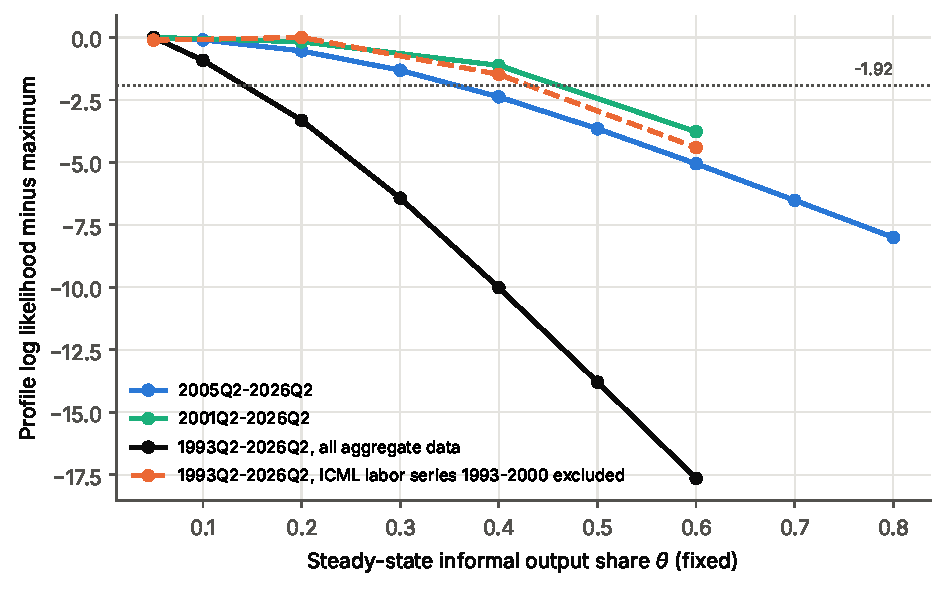
\includegraphics[width=0.85\textwidth]{fig_profiles.pdf}
\caption{Profile log likelihood of the steady-state informal share $\theta$, by sample. Values relative to the maximum of each profile; the dotted line marks $-1.92$.}
\label{fig:profiles}
\end{figure}

\begin{table}[H]
\centering
\caption{Profile log likelihood relative to its maximum.}
\label{tab:profiles}
\footnotesize
\begin{tabularx}{\textwidth}{Y rrrr}
\toprule
\textbf{Sample} & $\theta=0.05$ & $\theta=0.20$ & $\theta=0.40$ & $\theta=0.60$ \\
\midrule
1993Q2--2026Q2, all aggregate data & 0.00 & $-3.32$ & $-10.02$ & $-17.65$ \\
1993Q2--2026Q2, ICML informality 1993--2000 left out & 0.00 & $-3.93$ & $-13.82$ & $-18.76$ \\
1993Q2--2026Q2, ICML employment and informality 1993--2000 left out & $-0.11$ & 0.00 & $-1.48$ & $-4.41$ \\
2001Q2--2026Q2 & 0.00 & $-0.18$ & $-1.12$ & $-3.77$ \\
2005Q2--2026Q2 & 0.00 & $-0.54$ & $-2.38$ & $-5.06$ \\
\bottomrule
\end{tabularx}
\end{table}

With the full sample the likelihood is informative: it favors small informal shares and rejects values above about 0.15. The information comes from the 1993--2000 period, and specifically from the employment series. Leaving out the informality rate of those years does not change the profile; leaving out employment as well makes it nearly flat, as are the profiles of the samples that start in 2001 or 2005. In those samples the likelihood varies by less than 1.5 log points between $\theta=0.05$ and $\theta=0.40$, and it only begins to penalize the largest values.

The second check compares prior and posterior dispersion. With all aggregate data the posterior standard deviation of $\theta$ is 57\% of the prior one (median 0.18, 90\% interval 0.10--0.29), against 80\% when the 1993--2000 labor series are left out and 81\% in the 2005 sample.

The third check uses simulated data. The model is simulated at the posterior median of the 2005 sample with a true informal share of 0.45, ten points above the prior mean, over the same 85 quarters and with the same missing quarters, and re-estimated (posterior mode and Laplace standard deviation) in three replications. Table~\ref{tab:simulation} reports the results. With the six aggregates the estimate lies between 0.51 and 0.56, with a standard deviation of about 0.08, close to the prior's 0.10: the data do not recover the true value.

\begin{table}[H]
\centering
\caption{Recovery of a known informal share ($\theta=0.45$) in simulated data, 2005Q2--2026Q2.}
\label{tab:simulation}
\footnotesize
\begin{tabularx}{\textwidth}{Y rrr rrr}
\toprule
& \multicolumn{3}{c}{\textbf{Six aggregates}} & \multicolumn{3}{c}{\textbf{Plus relative earnings}} \\
\cmidrule(lr){2-4}\cmidrule(lr){5-7}
\textbf{Replication} & 1 & 2 & 3 & 1 & 2 & 3 \\
\midrule
Posterior mode of $\theta$ & 0.561 & 0.508 & 0.554 & 0.450 & 0.448 & 0.459 \\
Laplace standard deviation & 0.083 & 0.076 & 0.079 & 0.004 & 0.004 & 0.005 \\
Ratio to prior standard deviation & 0.83 & 0.76 & 0.79 & 0.04 & 0.04 & 0.05 \\
\bottomrule
\end{tabularx}
\end{table}

\subsection{Alternative technology}
\label{sec:alt-tech}

A frequent alternative in the shadow-economy literature lets the informal sector produce with labor only and decreasing returns, $Y_{i,t} = A_i X_t N_{i,t}^{\eta}$ \citep{IhrigMoe2004, ElginOztunali2012}. With that technology aggregate shocks change the relative return of the two types of work, and the informality rate responds to capital and to the trend shock. Estimated on the 2005 sample with $\eta$ free (prior mean 0.7), the profile likelihood of $\theta$ is as flat as with the common technology on the same sample: it falls by 2.1 log points between $\theta=0.10$ and $\theta=0.40$. A different technology does not solve the identification problem.

\subsection{An observable that identifies the level}

Proposition~\ref{prop:share} indicates what is missing: a direct measure of the earnings ratio $R_t$. In the labor-only model the observed ratio of informal income per worker to the mean wage of formal employees is
\begin{equation}
\ln R^{\mathrm{obs}}_t = \ln\frac{Y_{i,t}}{N_{i,t}} - \ln\Big((1-\alpha)\frac{Y_{f,t}}{N_{f,t}}\Big) + \ln(1+d_t^{\mathrm{nw}}) + b\,\mathbb{1}_{t\ge 2022Q1} + e^{R}_t,
\label{eq:earnings}
\end{equation}
where $\ln(1+d_t^{\mathrm{nw}})$ converts the wage reported by formal employees into the employer's labor cost using the statutory non-wage costs of Section~\ref{sec:data} (a constant wedge, $-\ln(1-\bar\tau)$ with $\bar\tau=0.25$, in a sensitivity), $b$ is a level shift for the change in the definition of informality and $e^{R}_t$ is measurement error. In log deviations the first two terms are $z^r_t + (\eta-1)\hat n_{i,t} - \alpha(\hat k_t - \mu_t - \hat n_{f,t})$, and their steady-state value is a function of $\theta$. With equal technologies the first two terms reduce to $\ln\tilde\rho + z^r_t$. The ratio can be computed from the household survey for every month since 2007 with the same classification of informality as the employment series. Equation \eqref{eq:earnings} enters the state space in levels and activates the shock $z^r_t$. In the simulation of Table~\ref{tab:simulation}, adding this observable recovers the true share with a standard deviation of half a percentage point.

In the labor-only model the earnings ratio depends on informal employment through $\eta$. If the informality rate entered only in changes, a very persistent deviation of the wedge could shift $\hat n_{i,t}$ and mimic a different $\theta$: in a first estimation the chains settled on different values of $\theta$ ($\hat R=1.57$). The labor-only estimates therefore observe the logit of the informality rate in levels, as a deviation from the logit of its sample mean with the quarter-of-year pattern removed, with an independent level error. This pins the state of the wedge in every quarter and removes the trade-off.

\subsection{Identification in the baseline model}
\label{sec:id-baseline}

Three checks are repeated for the baseline: the labor-only model with the informality rate in levels and the earnings observable.

\paragraph{Recovery of a known share.} Data are simulated from the baseline at its posterior median with a known steady-state share of 0.20 or 0.40, with the same length and missing quarters as the actual data, and $\theta$ is re-estimated (posterior mode and Laplace standard deviation) with and without the earnings observable (Table~\ref{tab:sim-labor-only}). Without earnings the estimate is roughly centered on the truth but its standard deviation is 41\%--46\% of the prior's. With earnings it is recovered within half a percentage point, with a standard deviation of 3\%--5\% of the prior's.

\begin{table}[H]
\centering
\caption{Recovery of a known steady-state share in data simulated from the baseline model (three replications per value).}
\label{tab:sim-labor-only}
\footnotesize
\begin{tabular}{c l c c c c}
\toprule
\textbf{True $\theta$} & \textbf{Observables} & \textbf{Mean mode} & \textbf{sd of modes} & \textbf{Laplace sd} & \textbf{Ratio to prior sd} \\
\midrule
\tableinput{tables/simulation_labor_only.tex}
\bottomrule
\end{tabular}
\end{table}

\paragraph{Profile likelihood in the data.} In the actual data the picture is different (Table~\ref{tab:profile-labor-only}). With or without earnings, the profile likelihood of the steady-state share is highest at the lowest value of the grid and falls monotonically. The likelihood alone does not pin down the steady state: the data can be matched with a low $\theta$ and with the economy away from its steady state for the whole sample, through levels that are not observed, such as the capital stock and total employment relative to their long-run values, which very persistent shocks can sustain. Observing the capital--output ratio built by perpetual inventory does not change this (Section~\ref{sec:results}).

\begin{table}[H]
\centering
\caption{Profile log likelihood of the steady-state share, baseline model with the constant wedge (relative to the maximum).}
\label{tab:profile-labor-only}
\footnotesize
\begin{tabular}{c c c}
\toprule
$\theta$ & \textbf{Aggregates only} & \textbf{With earnings ratio} \\
\midrule
\tableinput{tables/profile_labor_only.tex}
\bottomrule
\end{tabular}
\end{table}

\paragraph{What is identified: the path.} The quantity of interest is not the steady state but the informal share in each quarter, and Proposition~\ref{prop:share} shows that it depends on the informality rate and the earnings ratio of that quarter, both measured, and on $\alpha$. Table~\ref{tab:invariance} fixes the steady-state share at values between 0.10 and 0.40, re-optimizes every other parameter and recomputes the smoothed path. From 2007, when the earnings ratio is observed, the path changes by at most 0.3 percentage points; in the 1990s, where it is carried back by the model, by at most 1.4 points. Without the earnings observable nothing ties the path to a measured level, and the estimates without earnings are far from those with them (Section~\ref{sec:results}). The earnings ratio therefore identifies the level and trajectory of the output-share path. Before 2007 the path is identified with the information available for those years, the informality rate and the aggregates, and the model carries the earnings information back; the invariance table shows that this step moves the 1990s by at most 1.4 points. The steady-state parameter $\theta$ plays the role of a nuisance parameter: the likelihood does not pin it down on its own, its posterior combines the likelihood with the priors on the persistence of the shocks, and the path, which is the object of the paper, does not depend on it.

\begin{table}[H]
\centering
\caption{Informal share of output (\%) when the steady-state share is fixed and all other parameters are re-optimized, baseline model.}
\label{tab:invariance}
\footnotesize
\begin{tabular}{c c c c c c c}
\toprule
\textbf{Fixed $\theta$} & \textbf{1993Q2} & \textbf{2000Q4} & \textbf{2007Q2} & \textbf{2015Q2} & \textbf{2019Q2} & \textbf{2026Q2} \\
\midrule
\tableinput{tables/invariance.tex}
\bottomrule
\end{tabular}
\end{table}

Section~\ref{sec:results} applies the observable to the data.
